
%%%%%%%%%%%%%%%%%%%%%%%%%%%%%%%%%%%%%%%%%%%% Articolo - A4 - Portrait


%%%%%%%%%%%%%%%%%%%%%%%%%%%%%%%%%%%%%%%%%%%% preambolo

\documentclass[11pt]{article}

%%%%%%%%%%%%%%%%%%%%%%%%%%%%%%%%%%%%%%%%%%%% ackages
\usepackage[utf8]{inputenc}
\usepackage[italian]{babel}
\usepackage{multicol}

\usepackage{caption}
\captionsetup{justification=raggedright, singlelinecheck = false}
\setlength{\columnsep}{1cm}

\usepackage[margin=1in]{geometry}
\usepackage{amsfonts, amsmath, amssymb}
\usepackage[none]{hyphenat}
\usepackage{fancyhdr}
\usepackage{graphics}
\usepackage{float}
\usepackage[nottoc, notlot, notlof]{tocbibind}
\usepackage{pgf, tikz, pgfplots} 
\pgfplotsset{compat=1.15}
\usepackage{mathrsfs}
\usetikzlibrary{arrows, calc}
\usepackage{lipsum}

%%%%%%%%%%%%%%%%%%%%%%%%%%%%%%%%%%%%%%%%%%%% stitle pagina

\pagestyle{fancy}
\fancyhead{}
\fancyfoot{}
\fancyhead[L]{\small \MakeUppercase{ESERCIZI di matematica per il Liceo}}
\fancyhead[R]{\small \emph{prof. Diego Fantinelli}}
\fancyfoot[C]{\thepage}
\renewcommand{\headrulewidth}{0.5pt}
\renewcommand{\footrulewidth}{0.1pt}

\parindent 0ex
\setlength{\parindent}{0em}
\setlength{\parskip}{0em}
\renewcommand{\baselinestretch}{1.5}
\newcommand{\E}{\mathrm{e}}

%%%%%%%%%%%%%%%%%%%%%%%%%%%%%%%%%%%%%%%%%%%% title page

\begin{document}

\begin{titlepage}
\begin{center}
\vspace*{1cm}

\Large{\textbf{Diego Fantinelli}}\\
%\large{\textbf{- per il Liceo Scientifico -}}\\
\vfill
\line(1,0){400}\\[.5mm]
\huge{\textbf{ESERCIZI di Matematica}}\\[3mm]
\Large{\textbf{- per il Liceo Scientifico:  -}}\\[1mm]
\line(1,0){400}\\
\vfill
%{\scriptsize By Student Name}\\
%{\scriptsize Candidate \#} \\
%{\scriptsize \today} \\


\end{center}
\end{titlepage}

%%%%%%%%%%%%%%%%%%%%%%%%%%%%%%%%%%%%%%%%%%%% introduzione

\tableofcontents
\thispagestyle{empty}
\clearpage

\setcounter{page}{1}

\vspace*{1cm}
\section{Introduzione}
Il presente documento contiene le principali soluzioni per la formattazione di un testo scientifico, con particolare riferimento ai testi matematici, comprensivi di \emph{formule}, e caratteri speciali

\subsection{Come recuperare l'autostima}
Sed fringilla, neque sit amet maximus luctus, neque eros fermentum ipsum, nec hendrerit leo urna id urna. Pellentesque vel odio lobortis diam placerat porttitor non auctor leo.\\

\begin{multicols}{2}

\subsection{Formule in testo \emph{multicolonne}}
Orci varius natoque penatibus et magnis dis parturient montes, nascetur ridiculus mus. Integer pretium bibendum dolor eget interdum.\\[3mm]
\noindent
\vspace{10pt}
\begin{tikzpicture}
\begin{axis}[
    xmin=-11,xmax=11,
    ymin=-11,ymax=11,
    grid=both,
    grid style={line width=.1pt, draw=gray!10},
    major grid style={line width=.2pt,draw=gray!50},
    axis lines=middle,
    minor tick num=5,
    enlargelimits={abs=0.5},
    axis line style={-latex},
    ticklabel style={font=\tiny,fill=white},
    xlabel style={at={(ticklabel* cs:1)},anchor=north west},
    ylabel style={at={(ticklabel* cs:1)},anchor=south west}
]

\coordinate (O) at (0,0);
\node[fill=white,circle,inner sep=0pt] (O-label) at ($(O)+(-135:10pt)$) {};

\end{axis}
\end{tikzpicture}
\\
Sed ultrices mi a lacus vestibulum aliquet. Nam tincidunt dui in pellentesque hendrerit. Phasellus diam libero, laoreet eu varius sed, vulputate a orci. Etiam odio tortor, sagittis nec quam quis, iaculis ultrices purus. Nunc semper purus nec elit mattis.\\[4mm]
$\displaystyle{\lim \limits_{x \to \infty} \frac{f(b)-f(a)}{x-a}=f'(a)}$\\[4mm]
Sed ultrices mi a lacus vestibulum aliquet. Nam tincidunt dui in pellentesque hendrerit. Phasellus diam libero, laoreet eu varius sed, vulputate a orci. Etiam odio tortor, sagittis nec quam quis, iaculis ultrices purus. Nunc semper purus nec elit mattis.\\
\begin{equation}
	\displaystyle{\int_a^b{f(x) \,dx=\lim \limits_{x \to \infty} \sum \limits_{k=1}^{n}f(x_k) \cdot \Delta x}}
\end{equation}\\
Sed ultrices mi a lacus vestibulum aliquet. Nam tincidunt dui in pellentesque hendrerit. Phasellus diam libero, laoreet eu varius sed, vulputate a orci. Etiam odio tortor, sagittis nec quam quis, iaculis ultrices purus. Nunc semper purus nec elit mattis.\\[1.5mm]
\end{multicols}

%%%%%%%%%%%%%%%%%%%%%%%%%%%%%%%%%%%%%%%%%%%% sez. 2

\section{Classi Prime}

\subsection{Come inserire le formule matematiche}
Lorem ipsum dolor sit amet, consectetur adipiscing elit. Sed varius lacus eget magna elementum, quis ultricies justo vestibulum. Proin sed dolor vel est rhoncus tristique iaculis auctor mauris.\\[3mm]
$f(x)=(x-3)^2+ \displaystyle \frac{x}{2}$ ha dominio $\mathrm{D}_f:(-\infty,+\infty)$
e range $\mathrm{R}_f:\left[\frac{1}{2},\infty\right)$.\\

\subsection{Come inserire le formule matematiche}
Lorem ipsum dolor sit amet, consectetur adipiscing elit. Sed varius lacus eget magna elementum, quis ultricies justo vestibulum. Proin sed dolor vel est rhoncus tristique iaculis auctor mauris.\\[3mm]
$f(x)=(x-3)^2+ \displaystyle \frac{x}{2}$ ha dominio $\mathrm{D}_f:(-\infty,+\infty)$
e range $\mathrm{R}_f:\left[\frac{1}{2},\infty\right)$.\\

%%%%%%%%%%%%%%%%%%%%%%%%%%%%%%%%%%%%%%%%%%%% sez. 3
\newpage
\section{Classi Seconde}

\subsection{Come inserire le formule matematiche}
Lorem ipsum dolor sit amet, consectetur adipiscing elit. Sed varius lacus eget magna elementum, quis ultricies justo vestibulum. Proin sed dolor vel est rhoncus tristique iaculis auctor mauris.\\[3mm]
$f(x)=(x-3)^2+ \displaystyle \frac{x}{2}$ ha dominio $\mathrm{D}_f:(-\infty,+\infty)$
e range $\mathrm{R}_f:\left[\frac{1}{2},\infty\right)$.\\

%$\displaystyle{\lim \limits_{x \to \infty} \frac{f(b)-f(a)}{x-a}=f'(a)}$\\[1cm]

%%%%%%%%%%%%%%%%%%%%%%%%%%%%%%%%%%%%%%%%%%%% Equazioni utilizzando equation

\begin{equation}
	\displaystyle{\lim \limits_{x \to \infty} \frac{f(b)-f(a)}{x-a}=f'(a)}
\end{equation}\\[1cm]
\emph{integrali}
\begin{equation}
	\displaystyle{\int \limits_{a}^{b}x^2 \,dx=\left[\frac{x^3}{3}\right]_{a}^{b}=\frac{b^3}{3}-\frac{a^3}{3}}
\end{equation}\\[1cm]
\emph{Sommatorie}
\begin{equation}
	\displaystyle{\sum \limits_{n=1}^{\infty}ar^n=a+ar+ar^2+\cdots+ar^n}
\end{equation}\\[1cm]
\emph{Mix}
\begin{equation}
	\displaystyle{\int_a^b{f(x) \,dx=\lim \limits_{x \to \infty} \sum \limits_{k=1}^{n}f(x_k) \cdot \Delta x}}
\end{equation}\\[1cm]
\emph{Vettori}
\begin{equation}
	\displaystyle{\vec{v}=v_1 \vec{i}+v_2 \vec{j}=\langle v_1, v_2 \rangle}
\end{equation}

%%%%%%%%%%%%%%%%%%%%%%%%%%%%%%%%%%%%%%%%%%%% tabelle e arrays

\section{Classi Terze}
\begin{figure}[h!]
Nam tincidunt dui in pellentesque hendrerit. Phasellus diam libero, laoreet eu varius sed, vulputate a orci. Etiam odio tortor\\[5mm]
%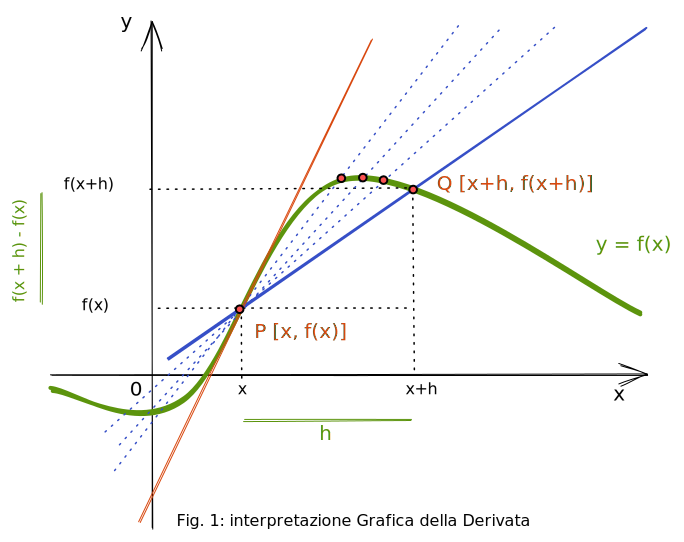
\includegraphics[width=0.7\textwidth]{Derivata}
\caption {\textit{Esempio di Rappresentazione grafica della derivata di una funzione}}
\end{figure}
\noindent
Nam tincidunt dui in pellentesque hendrerit. Phasellus diam libero, laoreet eu varius sed, vulputate a orci. Etiam odio tortor, sagittis nec quam quis, iaculis ultrices purus. Nunc semper purus nec elit mattis.\\

	\subsection{Tabelle e Arrays}
	\begin{table}[H]
%	\centering
	\caption{Relazione tra $f$ e $f'$.}
	\def\arraystretch{1.5}
	\begin{tabular}{c|c|r} % con |c| si definiscono le colonne e poi si separano le righe tra loro con \hline

	{$f(x)$} & {$f'(x)$}\\ \hline
	$x>0$ & La funzione $f(x)$ è \emph{crescente}. & prova 1\\
	\hline
	$x<0$ & La funzione $f(x)$ è \emph{decrescente}. & prova 2\\
	\hline	
	$x<0$ & La funzione $f(x)$ è \emph{costante}. & prova 3\\	
	\end{tabular}
		
	\end{table}

\section{Classi Quarte}
\section{Classe Quinte}

\section{Alcune \emph {Griglie per grafici}}
\subsection{Come inserire le formule matematiche}
Lorem ipsum dolor sit amet, consectetur adipiscing elit. Sed varius lacus eget magna elementum, quis ultricies justo vestibulum. Proin sed dolor vel est rhoncus tristique iaculis auctor mauris.\\[3mm]
$f(x)=(x-3)^2+ \displaystyle \frac{x}{2}$ ha dominio $\mathrm{D}_f:(-\infty,+\infty)$
e range $\mathrm{R}_f:\left[\frac{1}{2},\infty\right)$.\\

\begin{tikzpicture}
\begin{axis}[
    xmin=-11,xmax=11,
    ymin=-11,ymax=11,
    grid=both,
    grid style={line width=.1pt, draw=gray!10},
    major grid style={line width=.2pt,draw=gray!50},
    axis lines=middle,
    minor tick num=5,
    enlargelimits={abs=0.5},
    axis line style={latex-latex},
    ticklabel style={font=\tiny,fill=white},
    xlabel style={at={(ticklabel* cs:1)},anchor=north west},
    ylabel style={at={(ticklabel* cs:1)},anchor=south west}
]

\coordinate (O) at (0,0);
\node[fill=white,circle,inner sep=0pt] (O-label) at ($(O)+(-135:10pt)$) {};
\end{axis}

\begin{axis}[xshift=9cm,
    xmin=-11,xmax=11,
    ymin=-11,ymax=11,
    grid=both,
    axis lines=middle,
    minor tick num=5,
    enlargelimits={abs=0.5},
    axis line style={latex-latex},
    ticklabel style={font=\tiny,fill=white},
    xlabel style={at={(ticklabel* cs:1)},anchor=north west},
    ylabel style={at={(ticklabel* cs:1)},anchor=south west}
]

\coordinate (O) at (0,0);
\node[fill=white,circle,inner sep=0pt] (O-label) at ($(O)+(-135:10pt)$) {};

\end{axis}
\end{tikzpicture}

\vspace{1cm}

\begin{figure}[h!]
\begin{tikzpicture}
\begin{axis}[
	%xmin=0,xmax=5,
    %ymin=0,ymax=0.6,
    width=\textwidth,
	height=0.5\textwidth,
    grid=both,
    grid style={line width=.1pt, draw=gray!30},
    major grid style={line width=.2pt, draw=gray!50},
    axis lines=middle,
    minor tick num=5,
    enlargelimits={abs=0.5},
    axis line style={-latex},
    ticklabel style={font=\tiny,fill=white},
    xlabel=$x$,
    ylabel=$f(x)$
]

\end{axis}
\end{tikzpicture}
\caption{Griglia per Grafico Generico}
\end{figure}

%%%%%%%%%%%%%%%%%%%%%%%%%%%%%%%%%%%%%%%%%%%% Grafico di una Funzione

\newpage


\begin{figure}[h!]
\begin{tikzpicture}
\begin{axis}[
	%xmin=0,xmax=5,
    %ymin=0,ymax=0.6,
    width=\textwidth,
	height=0.5\textwidth,
    grid=both,
    grid style={line width=.1pt, draw=gray!10},
    major grid style={line width=.2pt, draw=gray!50},
    axis lines=middle,
    minor tick num=5,
    enlargelimits={abs=0.5},
    axis line style={-latex},
    ticklabel style={font=\tiny,fill=white},
    xlabel=$x$,
    ylabel=$f(x)$,
	legend entries={
        \small $y = 0.5x\E^{-x}$,
        \small $y=x\E^{-x}$,
        \small $y=2x\E^{-x}$,
        \small $y=3x\E^{-x}$
}
]
	\addplot[
	domain=0:5,
	thick,
	pink
	]
	{0.5*x*exp(-x)};
	
	\addplot[
	domain=0:5,
	thick,
	green
	]
	{x*exp(-x)};
	
	\addplot[
	domain=0:5,
	thick,
	dashdotted,
	blue
	]
	{2*x*exp(-x)};
	
	\addplot[
	domain=0:5,
	thick,
	black,
	dotted
	]
	{3*x*exp(-x)};
	
\end{axis}
\end{tikzpicture}
\caption{Il mio primo grafico}
\label{fig:primo-grafico}
\end{figure}

\appendix
%%\addcontentsline{toc}{chapter}{ALLEGATI}\\
%\addtocontents{toc}{\contentsline{chapter}{ALLEGATI}}\\
%%Il mio primo grafico con \emph{referencing} mostrato in Figura:\ref{primo-grafico}\\
%%\addtocontents{toc}{\contentsline{chapter}{ALLEGATO:}{\quad B}}
%%\addcontentsline{toc}{chapter}{ALLEGATO: \quad}
%
\newpage
\thispagestyle{fancy}
\fancyhead{}
\fancyfoot{}
\fancyhead[L]{\small \MakeUppercase{ALLEGATI}}
\fancyfoot[C]{\thepage}

\section*{ALLEGATI}
\subsection*{Allegato A - Integrali Indefiniti e Definiti}
\lipsum[4]
\newpage
\subsection*{Allegato B - Le Derivate}

\lipsum[2]
\newpage
\subsection*{Allegato C - Le Derivate di Ordine Superiore}

\lipsum[3]

%\lipsum[4]
%
%\section{Turorial Derivate}
%\lipsum[3]

\end{document}
